%\documentclass{svjour3}                     % onecolumn (standard format)
%\documentclass[smallcondensed]{svjour3}     % onecolumn (ditto)
\documentclass[smallextended, natbib]{svjour3}       % onecolumn (second format)
%\documentclass[twocolumn]{svjour3}          % twocolumn
%
\smartqed  % flush right qed marks, e.g. at end of proof
%
\usepackage{graphicx}
%\usepackage{cite},
\usepackage{amsmath}
\usepackage{mathptmx}  
\usepackage{subfigure}    % use Times fonts if available on your TeX system
%\usepackage{natbib}
%
% insert here the call for the packages your document requires
%\usepackage{latexsym}
% etc.
% please place your own definitions here and don't use \def but
% \newcommand{}{}
%B
% Insert the name of "your journal" with
% \journalname{myjournal}
%
\begin{document}

\title{The Alejandro Project: Testing the Target Contrast Signal Theory\thanks{ESRC grant?}
}
\subtitle{Replication and Generalisation}

\titlerunning{Testing the TCS Theory}        % if too long for running head

\author{Anna E. Hughes \and Anna Nowakowska \and Alasdair D. F. Clarke}

%\authorrunning{Short form of author list} % if too long for running head

\institute{F. Author \at
              first address \\
              Tel.: +123-45-678910\\
              Fax: +123-45-678910\\
              \email{fauthor@example.com}           %  \\
%             \emph{Present address:} of F. Author  %  if needed
           \and
           S. Author \at
              second address
}

\date{Received: date / Accepted: date}
% The correct dates will be entered by the editor

\maketitle

\begin{abstract}
Performance in visual search tasks is frequently summarised by ``search slopes'' - the additional cost in reaction time for each additional distractor. While search tasks with a  shallow search slopes are termed efficient (pop-out, parallel, feature), there is no clear dichotomy between efficient and inefficient (serial, conjunction) search. Indeed, a range of search slopes are observed in empirical data. The Target Contrast Signal (TCS) Theory is a rare example of quantitative model that attempts to predict search slopes for efficient visual search. In particular, the search slope in a double-feature search (where the target differs in both colour and shape from the distractors) can be estimated from the slopes of the associated single-feature searches. This estimating is done be using a contrast combination model, and previous work shows that a collinear contrast integration model outperformed other options. In our work, we extend the TCS to a Bayesian multi-level framework. We demonstrate that moving from using a normal distribution to a shifted-lognormal allows for a better fit of previously published data, and in doing so, we show that previous datasets are not sufficient to distinguish between the various contrast combination models that had been considered. We will conduct experiments that attempt to replicate the key original findings, with some changes to help distinguish between theories. 

\keywords{Visual search \and  Efficient search \and Parallel processing}

\end{abstract}

\section{Introduction}
\label{intro}

Visual search, where participants are asked to find a target within a cluttered scene, has been extensively studied within psychology. Several models have been developed that can generate testable predictions about how different types of distractors and targets affect search efficiency. One of the key distinctions in the field has been between efficient (also referred to as parallel or pop-out) and inefficient (serial) search. These are often studied in the context of the regression slope between the number of distracters and mean reaction time, which has been termed the \textit{search slope}. When the search slope is shallow (usually positive, but sometimes negative), the search is called efficient or parallel, and the addition of more non-target distracters has little impact on an observers difficulty in finding a target. When the slope is steeper, each additional distracter has a noticeable impact on increasing difficulty, and the search is described as inefficient or serial. 

The two most studied families of models of visual search include bottom-up models (also known as visual saliency models) and top-down models. Saliency models rest on the assumption that fixations are directed to objects or locations that are most dissimilar to the background or other objects in the visual display \citep{itti2000saliency, itti1998model, koch1987shifts}. While the original saliency model was able to predict fixation allocation in a visual search task above chance \citep{parkhurst2002modeling}, further research demonstrated that a comparable level of performance could be achieved using a simple central fixation bias heuristic \citep{tatler2007central}. The saliency models have since been extended and improved (see for example \cite{zhang2008sun}): however, the main issue with this family of models remains their limited usability in complex real-life search arrays \citep{tatler2011eye, koehler2014saliency}. In addition, in most instances of visual search, the target is clearly defined (i.e. the goal is to find a specific object) and inspecting the most salient areas of the display may in these cases be inefficient.

Another class of models are based around Feature Integration Theory \citep{treisman1980feature}, which has been modified and extended by Wolfe in the Guided Search Model \citep{wolfe1989guided,wolfe2014approaches}. These models combine top-down influences (how closely an item resembles the observer's goal) with bottom-up image properties. For example, if one's goal (top-down processing) is to find a red horizontal bar, all the red and horizontal items in a visual search display will be given greater weight than distractors (e.g. vertical and blue items) in the model. The salience of a given object in the display (how distinctive it is from the surrounding objects) also activates bottom-up processing. For instance, a blue item among red items is ranked higher than red among orange items. Combining bottom-up and top-down sources of activation generates an activation map which generates a prediction of the order in which stimuli are processed in visual search. Thus, these models aim to produce a representation of the visual properties of the distractors at each location in the visual field. 
 
However, more recent work has taken a different approach, focusing solely on representing the difference between targets and distractors. For example, in work on eye movement patterns, it has been proposed that performance in inefficient (serial) visual search is mostly determined by the size of the `functional viewing field', whose size varies as a function of target-distractor similarity \citep{hulleman2017brink}. 

The Target Contrast Signal (TCS) Theory \citep{lleras2020target} aims to provide a unifying, quantitative framework that can make behavioural predictions based on this general assumption. TCS proposes that behaviour is determined by comparing the target template (held in memory) with every element present in the scene in parallel. This allows the visual system to reject peripheral non-targets quickly; the speed at which items are evaluated is determined by how different the item is from the template through an evidence accumulation process (formally, the slope of the logarithmic function is assumed to be inversely proportional to the overall magnitude of the contrast signal between the target and distractor). The model thus focuses on an initial, efficient processing stage of search; if sufficient evidence is not accumulated during this process, the model posits that a second stage is entered, where attention is deployed serially. TCS has been successful in predicting a number of empirical results, including search performance in heterogeneous scenes based on parameters estimated in homogeneous scenes, both with artificial stimuli \citep{buetti2016towards,lleras2019predicting} and with real-world objects visualised on a computer display \citep{wang2017predicting}. 
 
The original version of the TCS theory is given below:
\begin{equation}
\hat{RT} = a + \sum_{j=1}^{L}(D_j-D_{j-1})\log{\left( N_T-\left(\sum_{i=1}^{j-1}N_i\right)I_{[2,\infty]}(L)+1\right)}
\label{eq:tcs}
\end{equation}

This is essentially log-linear model in the number of distractors. The intercept, $a$, corresponds to stimuli in which only the target is present and there are no distractors. $L$ represents the number of different types of distractors present in the display, while $N_i$ represents the number of individual distractors present of type $i$. $N_T$ is the total number of distractors, i.e., $N_T = \sum_{i=1}^{L}N_i$. Finally, $I_{[2, \infty]}$ is an index function that equals 0 when there $L<2$, and 1 otherwise\footnote{Note: Equation 1 in \cite{lleras2020target} had $j$ here rather than $L$. The current version is correct.}. In our paper, we will follow \cite{buetti2019predicting} and only consider the specific case of $L=1$, of a target among a homogeneous set of distractors  As such, the Equation \ref{eq:tcs} simplifies to:

\begin{equation}
\hat{RT} = a + D\log(N_T+1)
\label{eq:loglin}
\end{equation}

The core idea in \cite{buetti2019predicting} was \ldots

\begin{table}[h]
\centering
\begin{tabular}{ r|ccc } 
reference & overview\\
 \hline 
\cite{buetti2016towards} & \\
\cite{wang2017predicting} & \\
\cite{buetti2019predicting} & \\
\cite{lleras2020target} & \\
\end{tabular}
\caption{An overview of work on the Target Contrast Signal Theory}
\label{tab:tcs_overview}
\end{table}

\paragraph{Limitations, and extending basic stimuli} While results to date for TCS appear promising, they remain relatively preliminary, being tested by only one research group so far. There remains a great deal of scope for extending beyond the parameters tested to date (such as the number of distractors) in order to test the robustness and generalisability of the model. In addition, there are some predictions of the model, including its ability to explain search asymmetries, that have yet to be empirically confirmed \citep{lleras2020target}.

\paragraph{Within subjects}
In addition, in all implementations of TCS so far, predictions of search efficiency (e.g. in heterogeneous scenes) have been made on the average of a group of participants, using data from a different group performing a different task (e.g. searching in homogeneous scenes). Thus, we know that TCS can replicate group-level averages between subjects in search well, but we do not know whether it is also able to make predictions at the individual level. This is particularly important given that conclusions based on aggregate data can be different from those that take individual differences into account; in one study where participants searched for a target in an array of randomly oriented line segments, aggregating the data suggested that participants were using a stochastic search model. However, when considering each participant individually, it became clear that there was a high level of heterogeneity in responses, with some participants performing close to optimally, and others actually performing worse than chance \citep{nowakowska2017human}. Similarly striking variability has also been reported in other search studies \citep{irons2016choosing, irons2018characterizing}. 

\paragraph{Conclusion to introduction} 
In the current manuscript, we focus on replicating and extending findings from \cite{buetti2019predicting}. Here, participants searched for a target in a scene of homogeneous distractors. First, parallel search efficiency (measured by the logarithmic search slope) was estimated for cases where the distractors varied from the target in one dimension: either colour (e.g. a cyan target being searched for in either yellow, blue or orange distractors) or shape (e.g. a semicircle target in either circle, diamond or triangle distractors). New participants then searched for the same targets in displays where the distractors were compounds, differing from the target in both colour and shape (e.g. searching for a cyan semicircle in either blue circles, orange diamonds or yellow triangles). Figure \ref{fig:buetti2019_stimulus} shows example stimuli from their paper. The logarithmic search slopes in the initial experiments were then used to predict the logarithmic slopes and reaction times using a number of models. The authors found that the best model was a 'collinear contrast integration model' where the distinctiveness scores were summed along each attribute in the unidimensional experiments, creating an overall contrast score that was used for compound stimuli predictions.

\begin{figure}
\centering
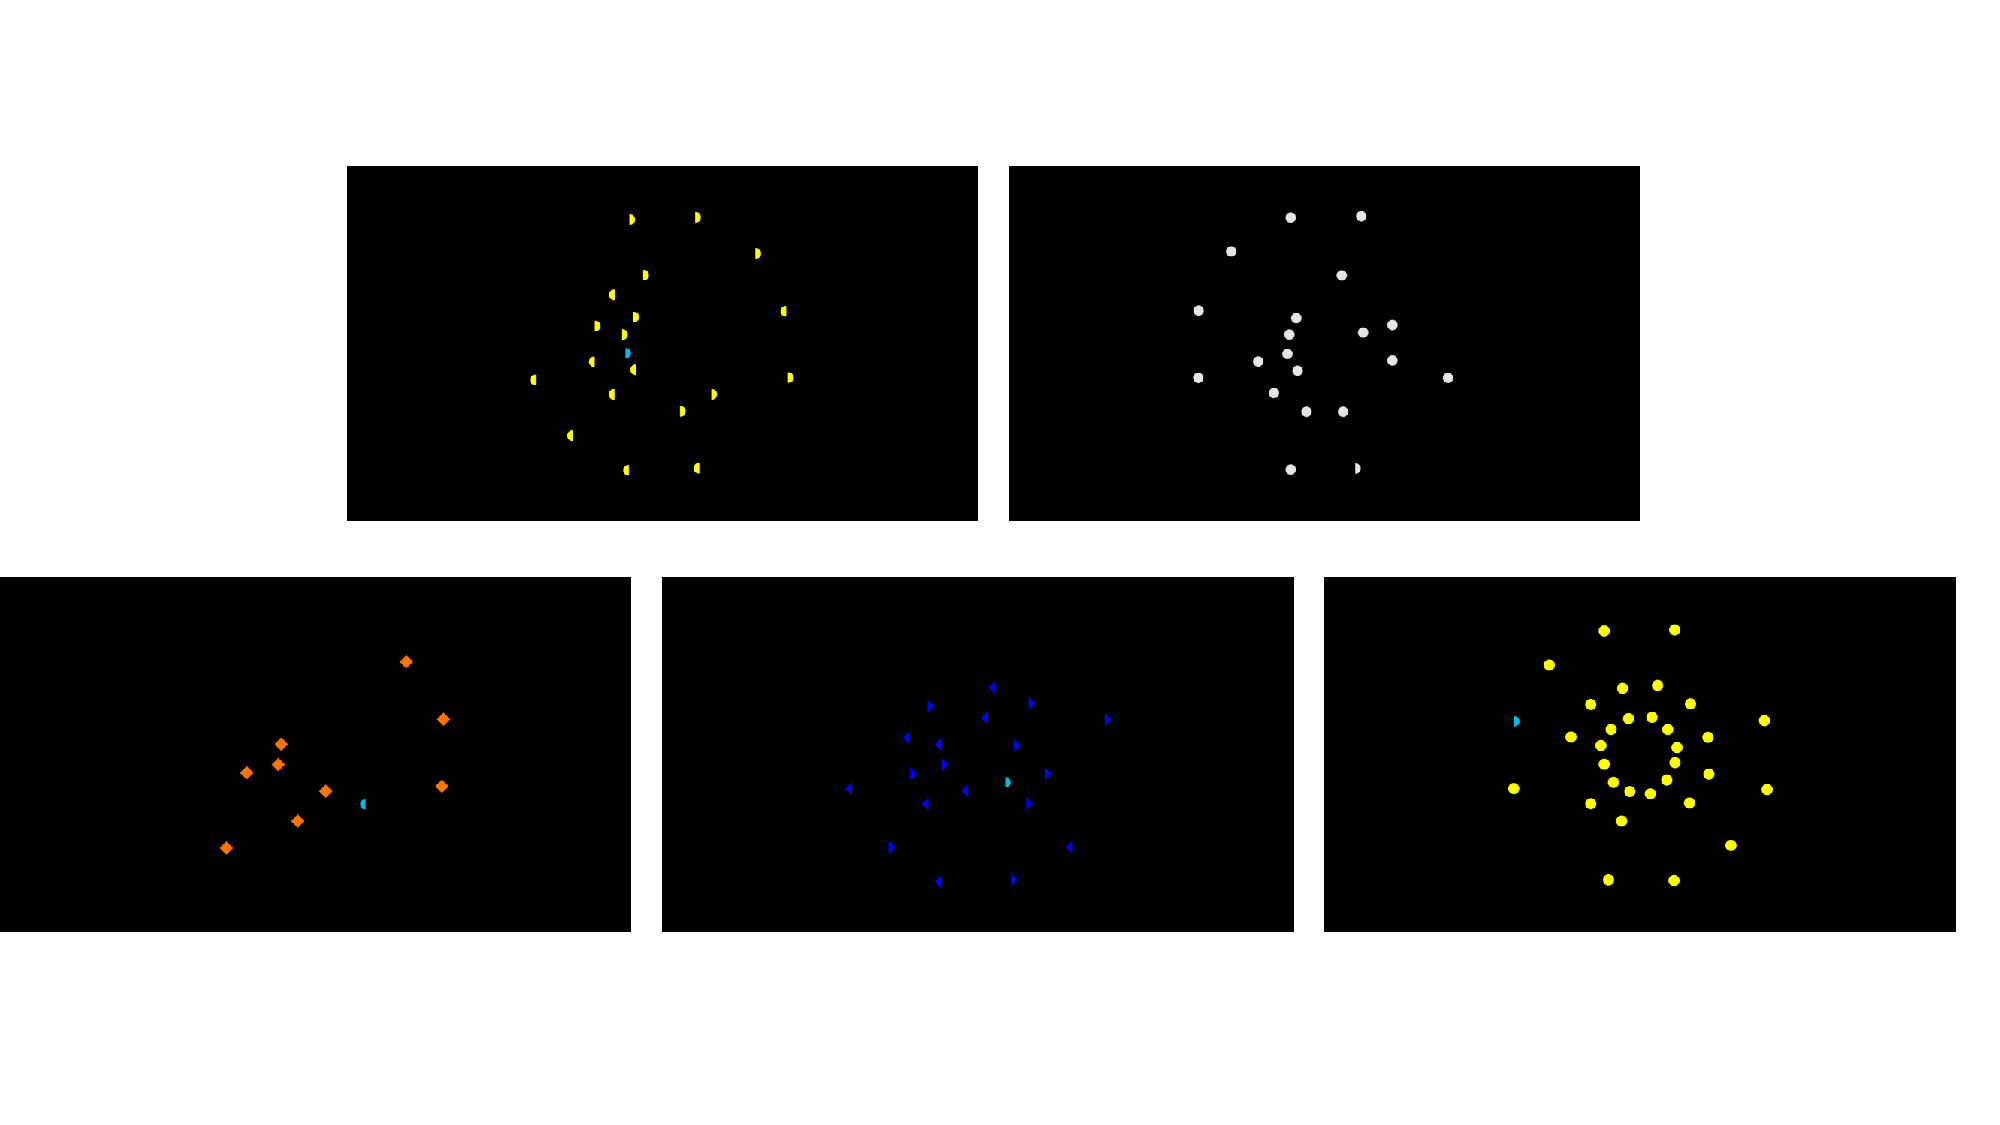
\includegraphics[width=\textwidth]{../plots/example_stimuli_figure.pdf}
\caption{Example stimuli from \cite{buetti2019predicting} Top left: Expt 1A. Here, the target is a blue semicircle within a set of homogeneous (yellow semicircle) distractors. Top right: Expt 1B. The target is a grey semicircle in circular grey distractors. Bottom left: Expt 2A. The target is a blue semicircle in orange diamond distractors. Bottom middle: Expt 2B. The target is a blue semicircle in dark blue triangle distractors. Bottom right: Expt 2C. The target is a blue semicircle in yellow circular distractors.}
\label{fig:buetti2019_stimulus}
\end{figure}

\paragraph{Overview of the current study}
We first run a replication of \cite{buetti2019predicting}, in an online, within-subjects study. This design allows us to extend the modelling, both incorporating a multi-level design to predict within-subjects effects and by utilising a Bayesian generalised linear model framework to better represent the distribution of responses (e.g. avoiding predicting negative reaction times, accounting for uncertainty in model predictions). We  also carry out a direct analytical replication using the same methods as in \cite{buetti2019predicting} allowing us to ask whether the choice of analysis affects the results.

\section{The Target Contrast Model}
\label{sec:reansalysis}

We first describe the original Target Contrast Model, as presented in \cite{buetti2019predicting} and verify that we can succesfully replicate the original analysis (see Supplementary Materials). This is followed by Section \ref{sec:reanalysis} in which we detail our proposed modifications and show how they change the interpretation of the data collected by \cite{buetti2019predicting}.

\subsection{TCS modelling overview} 

In Experiment 1a of \cite{buetti2019predicting}, participants searched for a cyan semicircle target among blue, yellow or orange semicircular distractors i.e. they searched for a target that differed from the distractors by a \textit{single feature} (colour). The experiment was then repeated (1b) using a different single feature (shape, with participants searching for the semicircular target within triangle, circle or diamond distractors). In Experiments 2a, 2b and 2c, participants again searched for a cyan semicircle, but this time, the distractors differed in both shape and colour. We will refer to these conditions as \textit{double features}. Note, unlike in standard conjunction searches, in this paradigm, the distractors are all identical with respect to these features (i.e, orange triangles). Examples of all these stimuli are shown in Figure \ref{fig:buetti2019_stimulus}.

The \textit{Target Signal Contrast} theory is built around a linear model for predicting mean reaction times from the logarithm of the number of distractors (see Equation \ref{eq:loglin}). In particular, the TCS theory allows us to predict the value of the logarithmic slope, $D_\text{c,s}$, in this condition based on the corresponding $D_j$ in the single feature search experiments. 

\subsubsection{Calculating the intercept, $a$, and the logarithmic slope parameter, $D_i$}
\label{sec:fitting_D}

Experiments 1a and 1b (referred to jointly as Experiment 1) were used to calculate the logarithmic slope parameter $D_i$. In both experiments, the number of distractors varied, allowing the data to be used to fit a log-linear model for reaction times, where reaction times increase logarithmically with $N_T$, the number of distractors. (See Equation \ref{eq:loglin}.) In the original model the error distribution was assumed to be normal. Thus the results of Experiment 1 were used to calculate $D_i$, for each type of distractor. When colour varied, we will refer to $D_c$, for $c=1,2,3$. Similarly for shape we will denote this ($D_s$), and the compound features are denoted as ($D_{c,s}$). 

Fitting the model specified in Equation \ref{eq:loglin} to the data, we obtain the values for $D_c$ and $D_s$ given in Table \ref{tab:reimp_Dc_Ds}. As can be seen, the more similar the distractors are to the target, the steeper the slope parameter is. 

\begin{table}[h]
\centering
\begin{tabular}{ ccc|ccc } 
feature & $D_c$ & $a$ & feature & $D_s$ & $a$\\
 \hline 
blue & 76.8 & 575.1 & triangle & 141.1 & 551.6\\
yellow & 16.0 & 575.1 & diamond & 77.2 & 537.7\\
orange & 9.8 & 575.1 & circle & 62.1& 555.8\\
\end{tabular}
\caption{A table of $D_i$ values for Experiment 1a and 1b}
\label{tab:reimp_Dc_Ds}
\end{table}

As $a$ is the intercept in our model, it represents how long observers take to find a target when $N_T = 0$, i.e., there are no distractors. As such, it should be independent of both shape and colour. However, this leads to some ambiguity in how $a$ should be defined; in \cite{buetti2019predicting}, $a$ was calculated for each feature in each sub-experiment (e.g. Experiments 1a, 1b, 2a, 2b, 2c; see Table \ref{tab:reimp_Dc_Ds}). Here, we follow that method in order to replicate their results exactly. Unfortunately, this leads to a situation in which the model's prediction of how long participants take to find a target when $N_T$ depends on the features of distractors that are not present in the stimulus! As such, in our proposed new version of the TCS theory, we will estimate $a$ at the level of an experiment (e.g. Experiments 1 and 2).

\subsubsection{Estimating $D_{c,s}$, the logarithmic slope parameter for compound features}

In the context of the current experiments, the core idea of TCS theory is that we can estimate the logarithmic slope parameter for a double feature visual search from the slopes parameters in the two independent single feature searches. I.e., $D_{c,s} = f(D_c, D_s)$. \cite{buetti2019predicting} tested three different models for predicting $D$ for compound colour-shape stimuli. The best feature guidance model (Equation \ref{eq:bestfeature}) suggests that when the target and lures differ in two dimensions, participants will choose to attend to whichever feature dimension is the most discriminable (i.e. has the smallest $D$ value):

\begin{equation}
D_\text{c,s} = \text{min}\left(D_\text{c}, D_\text{s}\right)
\label{eq:bestfeature}
\end{equation}

The orthogonal contrast combination model instead suggests that independent feature dimensions comprise a multidimensional space, where an object can be described by the overall vector in this space, and thus $\mathrm{D_{c,s}}$ can be represented as\footnote{Note: there is a small mistake in Equation 4 in \cite{buetti2019predicting}. The version given here is correct.}:

\begin{equation}
D_\text{c,s} = \frac{1}{\sqrt{\frac{1}{(D_\text{c})^2 + (D_\text{s})^2}}}
\label{eq:orthogonalcontrast}
\end{equation}

Finally, the collinear contrast integration model also assumes independence of feature dimensions, but assumes that while the visual features create a multidimensional space, the contrast between them is unidimensional. As $D$ is assumed to be inversely proportional to contrast, the equation can be written as follows:

\begin{equation}
\frac{1}{D_\text{c,s}} = \frac{1}{D_\text{c}} + \frac{1}{D_\text{s}}
\label{eq:collinearcontrast}
\end{equation}

\cite{buetti2019predicting} found that with their dataset, the collinear contrast integration model was best able to predict $D_{c,s}$ from $D_c$ and $D_s$, with $R^2 = 0.915$. We verified we were able to replicate this result using the dataset available on OSF (https://osf.io/f3m24/)\footnote{downloaded on 28th August 2020} and using the exclusion criteria originally applied; see Figure \ref{fig:comp_rep} (left panel) and \textit{Supplementary Materials} for details.

\begin{figure}
\centering
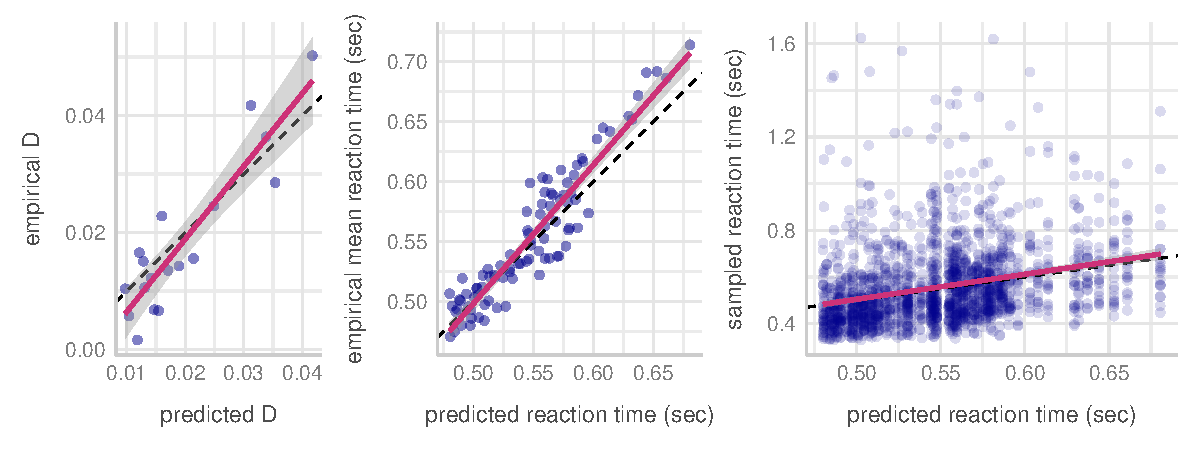
\includegraphics[width=\textwidth]{../plots/computational_replication.pdf}
\caption{(left) The collinear method for calculating $D$ offers a good prediction. (centre) Using the TCS to predict reaction times. (right) Each dot now represents a randomly sampled reaction time from an observer.}
\label{fig:comp_rep}
\end{figure}

\subsubsection{Estimating mean reaction times}

Finally, we can use Equation \ref{eq:loglin} to predict mean reaction times. As can be seen in  Figure \ref{fig:comp_rep} (centre panel), these predictions are essentially identical to the empirical RT results: $R^2 = 0.93\%$.

\subsubsection{Discussion}

While TCS theory offers a good prediction of search slopes and corresponding mean reaction times for double feature search, there are two related limitations. Firstly, it is unable to account for individual differences between observers, only the changes to the sample average. Secondly, it cannot account for the distribution of reaction times over multiple trials. Figure \ref{fig:comp_rep} (right panel) shows clearly that these factors generate high levels of variability within the individual trial-level data. To address these issues, we propose a second version of the TCS that make use of multi-level modelling techniques.

It is also worth noting that relying simply on $R^2$ values may give a misleading view of the accuracy of the TCS model. Figure \ref{fig:comp_rep_conditions} (top) shows the predicted RTs (pink line) for three conditions from Experiment 2 (a, b and c) of \cite{buetti2019predicting}, plotted next to the mean of means for each condition. It is clear that for at least some conditions, the TCS model is doing a poor job of predicting the empirical data, even when allowing quite rigid constraints on the model; for example, the intercept ($a$) is set at the level of each sub-experiment and thus would be expected to be perfect. To some extent, this could reflect the fact that the $R^2$ measure of goodness-of-fit simply measures how tightly clustered the points are around a line with arbitrary intercept and slope. It is possible therefore for the $R^2$ value to be high, but for the line to deviate significantly from an intercept of 0 and a slope of 1, which is the unity line required for the predictions to be a good match to the empirical data. For our reimplementation of the TCS model, we will therefore assess model fit by computing the log marginal likelihoods via bridge sampling. This directly assesses how well our values of $D_{c,s}$ are able to predict RTs, avoiding the issues with the $R^2$ measure.

Finally, if we look at the different predictions made by the three proposed feature combination models, we can see that in most of the parameter space explored in \cite{buetti2019predicting}, the models all make very similar predictions (Figure \ref{fig:comp_rep_conditions}, bottom). In Experiment 2, we are only able to discriminate between models in the \textit{blue} conditions, whereas in the \textit{yellow} and \textit{orange} conditions, they make essentially identical predictions. As such, if we want to distinguish between these three models, we will have to combinations of features that lead to larger target-distractor combinations. We will therefore use yellow, green and blue distractors in our replication study where participants are required to find a cyan target, hopefully generating a wider range of target-distractor differences.

\begin{figure}
\centering
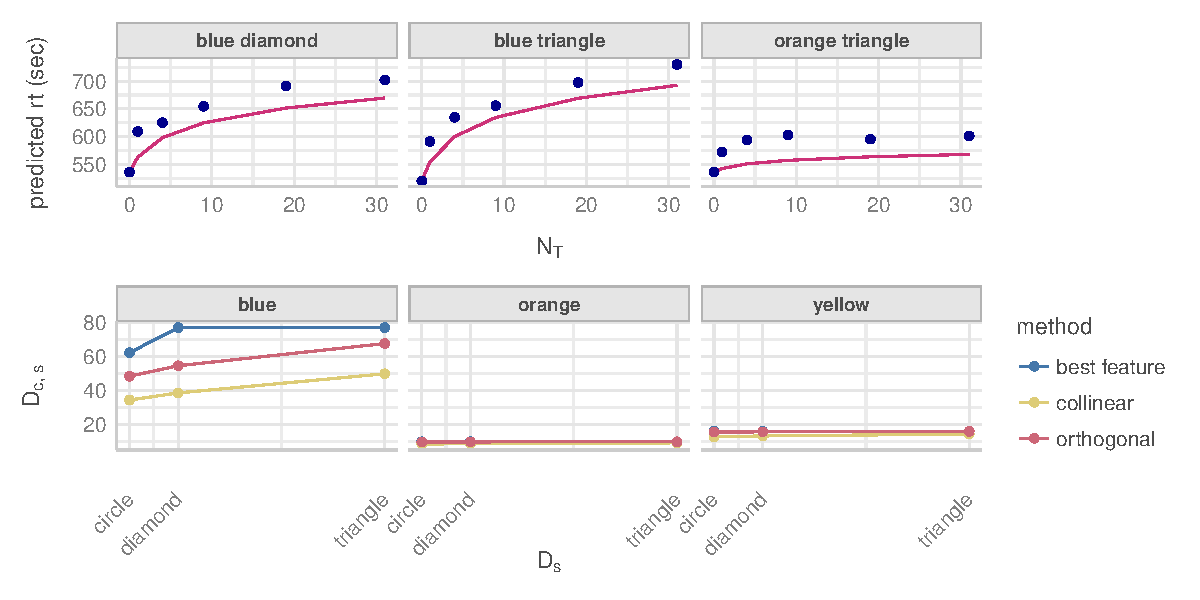
\includegraphics[width=\textwidth]{../plots/computational_replication_issues.pdf}
\caption{(top) Three conditions from Experiment 2. Blue dots represent the mean of means for each condition, while the line shows the prediction of the TCS theory. (bottom) Estimates of $D_{c,s}$ for the different colours and shape from \cite{buetti2019predicting}. As can be seen, in two of the three colour conditions, we are unable to distinguish between best feature, collinear or orthogonal contrast models.}
\label{fig:comp_rep_conditions}
\end{figure}

\subsection{A multi-level TCS}
\label{sec:reanalysis}

Switching from a linear regression model to a multi-level model will allow us to compute $D$ for each participant, while simultaneously estimating the trial-to-trial variance. We also switch from a frequentist to Bayesian framework, as this allows us to naturally account for the uncertainty in the model's predictions.

However, switching from linear regression to a multi-level model raises the problem of which distribution to use for modelling reaction times. Using a normal distribution is unlikely to be satisfactory, as it is unable to account for the skew frequently seen in reaction time distributions, and also allows the possibility of negative reaction times. We can account for both of these problems by using a log-normal distribution, $\text{rt} ~ \text{lognormal}(\mu, \sigma))$. We will also test whether a slightly more complex extension of this model, the \textit{shifted lognormal} model (which allows the distribution to be offset to the right i.e. mimicking the patterns seen in reaction time data, where valid responses begin at around 100ms) offers any improvement in model fit.

Throughout the paper, we will make use of the $53\%$ and $97\%$ \textit{highest posterior density intervals} (HPDI) to summarise probability distributions. These can be thought of as the smallest interval that, given our data and assumptions, contain $53\%$ and $97\%$ of the probability mass. 

Finally, when comparing models, we discuss that $R^2$ value on its own is not an adequate measure of the goodness-of-fit of the model, and that the match to the unity line also needs to be considered. We suggest adjustments to the original models proposed by \cite{buetti2019predicting} to improve the predictive power of the TCS model: namely that we should assess goodness-of-fit of the model, using bridge sampling to calculate the log marginal likelihoods.

\subsubsection{Calculating the logarithmic slope parameter, $D_i$}

We began in a similar fashion to section \ref{sec:fitting_D}, although this time, we fitted each model three times using a (i) normal, (ii) lognormal, and (iii) shifted lognormal distribution (please see Supplementary Materials for full details of out modelling approach, including prior predictive checks and model fit diagnostics). The three models were compared using bridge sampling to calculate the log marginal likelihoods, and the results showed that the shifted-lognormal model (illustrated in Figure \ref{fig:buetti2019_a1}) was given $100\%$ of the weight\footnote{we also tested a version of the shifted lognormal model that did not use the logarithm of the number of distractors i.e. testing this assumption of the TCS model, but found no support for this model being better: see Supplementary Materials for further details.}. Therefore, we used only this model for the rest of the analysis. 

\begin{figure}
\centering
\subfigure{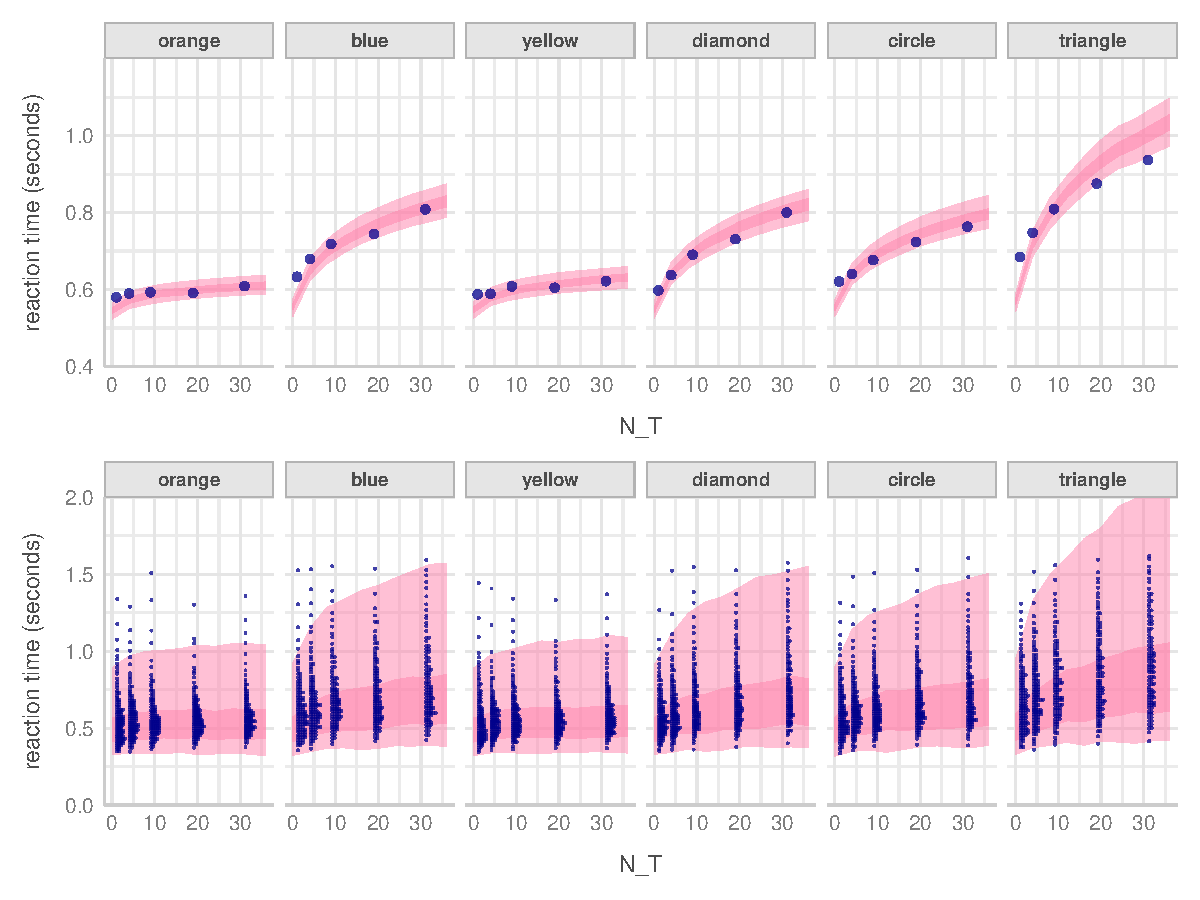
\includegraphics[width=\textwidth]{../plots/bayes_buetti_refit.pdf}}
\caption{(\textit{top}) The shaded regions show the model's estimate ($53\%$ and $97\%$ intervals) of the average participant's mean reaction time, while the points show the empircal mean reaction time. (\textit{bottom}): The shaded regions now indicate the distribution of reaction times (over a new simulated group of participants) generated by the model. The points now represent the 100 quantiles from the empirical data.}
\label{fig:buetti2019_a1}
\end{figure}



\subsubsection{Estimating $D_{c,s}$, the logarithmic slope parameter for compound features}

The first step in predicting the values for $D_{c,s}$ is to extract the logarithmic slope parameters $D_c$ and $D_c$ from our model outlined above (Figure \ref{fig:buetti2019_D} (top)). This is the same as the original TCS, except this time we use 1000\footnote{check!} samples from the posterior distributions, rather than just the maximum likelihood fit. The then combine $D_c$ and $D_c$ using the best feature, orthogonal contrast, and collinear contrast integeration models to get three different predictions for $D_{c,s}$ . These are illustrated in Figure \ref{fig:buetti2019_D} (bottom).

\begin{figure}
\centering
\subfigure{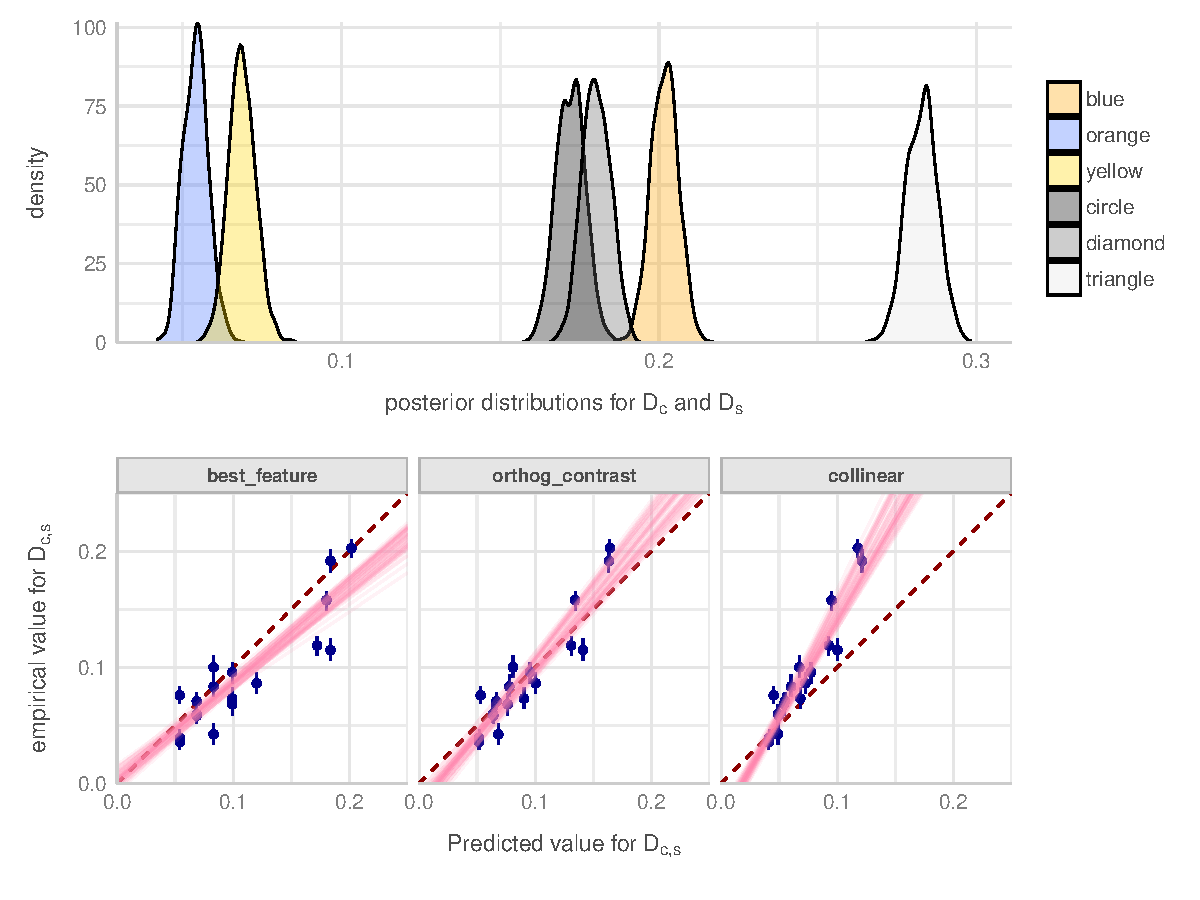
\includegraphics[width=\textwidth]{../plots/bayes_buetti_D.pdf}}
\caption{(\textit{top}) Posterior probability density functions for each $D_c$ and $D_s$ in Experiment 1. As with the original TCS model, when searching for a blue semicircle, triangular distractors are the hardest, while yellow and orange distractors are the eaiest.) (\textit{bottom}) Predicting $D_{c,s}$ from $D_c$ and $D_s$. Crosshairs indicate $97.5$ HPDI for estimates and predictions, while the pink region shows the HPDI for the best fit line. }
\label{fig:buetti2019_D}
\end{figure}

The $R^2$ values for the three approaches are shown in Table \ref{tab:reimp_D_r2}. We can see that as with the original model, we still find the \textit{best feature} is the worst of the three methods, at least in terms of the raw $R^2$ value. However, it is less clear which of the other two methods gives the best performance. While the collinear contrast approach offers the highest $R^2$ (0.824-0.963), it consistently predicts values that are too low. The orthogonal contrast method gives more accurate predictions, albiet with a slightly lower $R^2$ (0.739-0.944). As such, we propose a different method, (see below) to distiguish between these approaches. 

\begin{table}[h]
\centering
\begin{tabular}{ c|cc|ccc|c } 
Method & Intercept & Slope & $R^2$ & $R^2$ Lower & $R^2$ Upper & Model Weight\\
 \hline 
best feature & 0.003 & 0.831 & 0.752 & 0.545 & 0.927 & 34.0\%\\ 
orthogonal contrast & -0.019 & 1.206 & 0.856 & 0.739 & 0.944 & 33.6\%\\ 
collinear & -0.034 & 1.814	& 0.901 & 0.824 & 0.963 & 32.4\%\\
\end{tabular}
\caption{A table of $R^2$ values}
\label{tab:reimp_D_r2}
\end{table}

\subsubsection{Estimating other parameters and predicting reaction times}

Unlike the original TCS, before we can use the predicted values of $D_{c,s}$ to generate reaction times, we first have to estimate some additional parameters: 

\begin{itemize}	
\item $\alpha$ - the intercept for the shift\footnote{ndt} parameter.
\item $\phi_a$ - the random intercepts for the linear predictor for $\mu$.
\item $\phi_\alpha$ - the random intercepts for $a$.
\item $\sigma$ - the residual (trial-to-trial) variance. 
\end{itemize}

For the implementation presented here, in order to predict the data from Experiment 2 we will simply use the values for the above parameters obtained from Experiment 1. Once these have been set, we can use the specified model to generate the HPDI intervals for the expected average performance and the full distribution of reaction times over a number of simulated new observers (Figure \ref{fig:buetti2019_rt}).

\begin{figure}
\centering
\subfigure{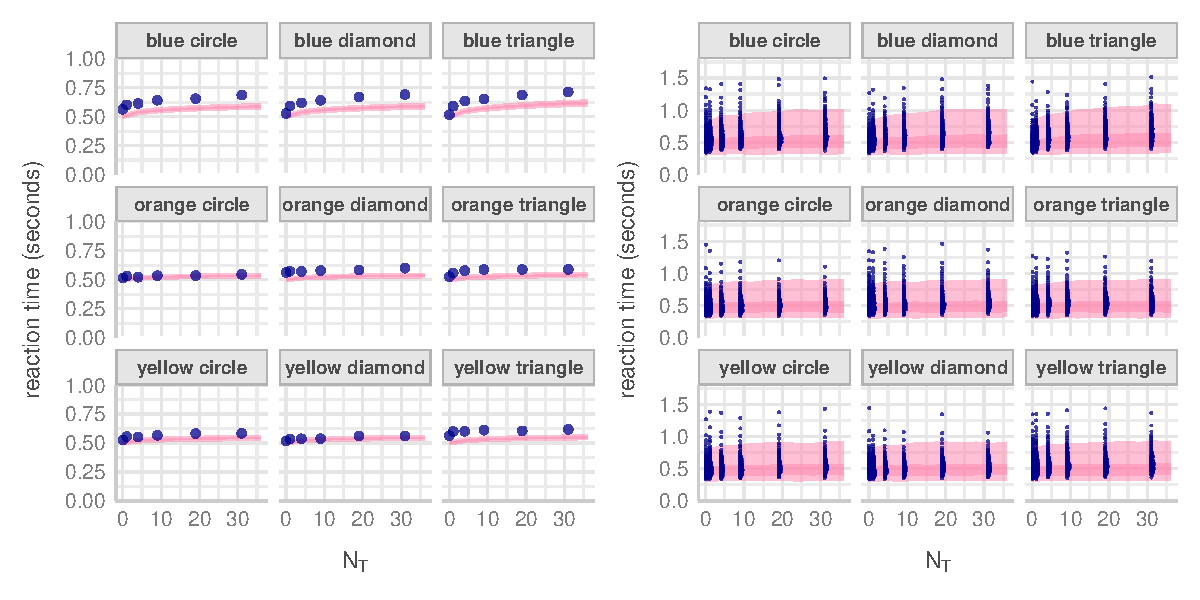
\includegraphics[width=\textwidth]{../plots/bayes_buetti_rt.pdf}}
\caption{(\textit{left}) HPDI and empirical mean reaction times for each condition in Experiment 2, using the collinear contrast integration model to predict D values. (\textit{right}) Similar, for the full distribution of reaction times over trials. }
\label{fig:buetti2019_rt}
\end{figure}

We can summarise how well the model predicts the mean reaction times (Figure \ref{fig:buetti2019_rt}, left) by repeatedly i) sampling from the posterior, ii) computing the predicted mean reaction times, iii) computing the $R^2$ statistic for the correlation between predicted and empirical mean reaction times (as done in \cite{buetti2019predicting}) and iv) calculating a measure of goodness-of-fit of the model predicting RTs from the $D_{c,s}$ values.

At first glance, our model appears to be offering a poorer fit with the the data than the original TCS. This is due to our decision to estimate $a$ (the intercept) from the Experiment 1 data, whereas \cite{buetti2019predicting} estimated three values for $a$, one for each sub-experiment, and these values were estimating from the Experiment 2 empirical data. With the within-subject design we propose for our replication study, this issue should not arise. Our new model gives us a HPDI of $[0.78, 0.83]$ for the $R^2$ value when fitting the best fit model using the $D_{c,s}$ predicted values from the collinear contrast integration method (see Table \ref{tab:reimp_D_r2}), which compares with the value of $R^2 = 0.93$ obtained for the original TCS.  

However, our goodness-of-fit measures showed that there was little difference between our models: the posterior model probability of the collinear contrast model was 32.4\%, compared to 33.6\% for the orthogonal contrast model and 34.0\% for the best feature model. There is therefore no strong evidence for one model over another. This contrasts with \cite{buetti2019predicting}, who concluded that the collinear contrast integration model offered the best fit to their data. They reasoned that this was due to the independence of the two features in their study, and they would not expect this result to generalize to integral dimensions\footnote{cite Garner for odd terminology?}, in which case they expect the \textit{orthogonal} contrast combination model to offer the best predictions. However, our analysis suggests that there is no strong evidence that any of the models tested is superior to the others. As we can see in Table \ref{tab:reimp_D_r2}, the $R^2$ values are very similar across methods. 

Overall, while our new model appears to fit slightly more poorly than the than the original method, as discussed above, it offers substantial improvements over the original model in terms of predicting the full distribution of reaction times over multiple trials and participants. In addition, as we discuss previously, the $R^2$ value may not capture goodness-of-fit optimally, and more sensitive goodness-of-fit metrics suggest that the models have equivalent predictive value.

\subsection{Discussion}

Our extension to a multi-level TCS model allows us to go beyond the original version and predict the full distribution of reaction times over samples of known, or new, observers. Moving from a normal to a shifted-lognormal distribution allows us to accurately model the skew seen in the empirical data, and avoid predicting negative response times. Our modelling has also highlighted other issues that we will address during our replication study: firstly, using a within-subjects design allows $a$ to be calculated in a more principled manner, and secondly, we will choose distractor features to give the highest possible $D$ sensitivity, and thus give us greater power to detect true differences between models.

\section{Hypotheses}

We plan an experiment to test the extent to which the original results in \cite{buetti2019predicting} replicate and generalise.

\subsection{Proposed Modifications to Experimental Design}

In order to better test the above, and increases sensitivity, we propose to make the following changes to the experiment described in \cite{buetti2019predicting}:

\begin{enumerate}
\item \textbf{Within-subjects design} This modification should give us greater power to detect differences between different models, as well as allowing us to investigate how individual differences in the single-feature task might explain differences in the double-feature task.
\\
\item \textbf{Increase target-distractor similarity} Our reanalysis of \cite{buetti2019predicting} indicates that the orange distractor condition does not distinguish well between different contrast models. We will therefore replace the orange distractor condition with a green distractor condition, which is more similar to the light blue target.
\\
\item \textbf{Increase number of distractors, and more peripheral distractors} The TCS model, if it is to be a useful predictor of human behaviour, should generalise beyond the conditions originally tested. We therefore will add an extra condition, with 43 distractors. This requires the addition of another ring of possible distractor positions compared to \cite{buetti2019predicting}, allowing the distractors in all conditions to be placed in more peripheral locations. 
\\
\item \textbf{Online data collection} This again tests the generalisability of the results obtained so far in laboratory conditions.
\end{enumerate}

\subsection{Registered Hypothesis}

\begin{enumerate}
\item \textbf{Shifted lognormal model} We hypothesise that a shifted lognormal model will give the best fit to our single-feature data, when compared to a lognormal and a normal model. \\
\item \textbf{Log-linear effect of $N_T$.} We will test the TCS model assumption that $N_T$ has a log-linear effect by testing models with and without the log of this term.\\ 
\item \textbf{Contrast model comparisons} We will test the hypothesis proposed by \citep{buetti2019predicting}: specifically, that the \textit{collinear contrast ingratiation model} outperforms the \textit{best feature guidance}, and \textit{orthogonal contrast combination models}.\\
\end{enumerate}

We will test each of these hypotheses by calculating the marginal likelihood of the relevant models, and then calculating the poster probabilities. This will give us a probability for each model that represents the likelihood that the model gives the best prediction. We will consider there to be evidence for one model over the others if a given model has a probability above 90\%. We will consider there to be strong evidence for one model over the others if that model has a posterior probability above 99\%.

\subsection{Planned Explorations}

We plan to investigate the effect of individual differences in this paradigm: to what extent performance in the single-feature task can predict performance in the double-feature task for a given individual (\cite{buetti2019predicting} were not able to investigate this due to the between-subjects design of their study). We plan to do this by specifying a more complex random effects structure for the model, that allows for individual differences across different slopes for different features. This allows us to then study the random effect correlation structure.  However, given these models can be challenging to fit, we will do this in an exploratory manner after carrying out our formally registered analysis.

\section{General Methods}

\subsection{Sample Size: Participants and Trials}

To determine our sample size, we carried out a simulation study to estimate the effect of reducing the number of trials and increasing the number of participants on our ability to accurately measure the $D_i$. While our reanalysis of \cite{buetti2019predicting}'s data is unable to distinguish between the three models of contrast combination, we believe that this is due to the feature values used in their study, rather than low statistical power from sampling (see above and Figure \ref{fig:comp_rep_conditions}). Therefore, we will base our sensitivity analysis around the width of the $97\%$ HPDI when estimating $D_{\text{blue}}$. We have chosen to look at this single feature level as it is clear from above that the blue distractor trials offer greater discrimination between the three contrast models.

We carried out our simulation sensitivity analysis by generating synthetic data from the shifted lognormal model outlined in Section \ref{sec:reanalysis}, Figure \ref{fig:buetti2019_a1}, for the blue distractor conditions. This was done for several different sample sizes, both in terms of number of trials and number of participants. For each synthetic dataset, we then refit the model and calculated the width of the $97\%$ HPDI (see Figure \ref{fig:power_plot}). F

\begin{figure}
\centering
\subfigure{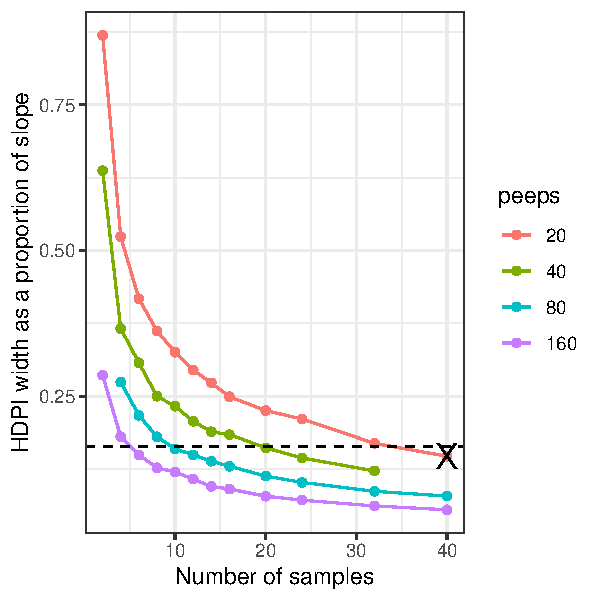
\includegraphics[width=\textwidth]{../plots/power_plot.pdf}}
\caption{Simulation sensitivity analysis, showing the 97\% HPDI width for the blue distractor condition in a shifted lognormal model, across different numbers of trials and participants. }
\label{fig:power_plot}
\end{figure}

As we are moving from the within-subjects design used by \cite{buetti2019predicting} to a within-subjects design in which each participant sees all combinations of features, we prefer to decrease the number of trials per person $\times$ condition from 40 to six. Increasing the number of participants from 20 to 80 will allow us to maintain sufficient accurcay in the estimating of logarithmic search slopes. 

Ethics?

\subsection{Stimuli}

The targets and distractors were randomly assigned to the display based on an invisible grid. Within each quadrant of the screen, there were three 'spokes' each with four possible target positions (starting from the centre of the screen and moving outwards), creating 48 different target positions in total, in four concentric circles. A small amount of jitter was added to each possible position to make the target locations less predictable.

\textbf{Distractor and target types:} we replicated the distractor types used in \cite{buetti2019predicting}, apart from that we changed one distractor colour (from orange to green) to allow us to discriminate better between different models of the data (see above). There were six single-feature conditions (yellow, green and blue distractors and triangle, circle and diamond distractors) and nine double-feature conditions (all possible pairings of the single-feature conditions). The target was always a light blue semicircle, except in the trials where the distractors were single-feature shapes (triangles, circles and diamonds) in which case the target was a white semicircle.

\textbf{Set sizes:} we ran all the distractor set sizes used in \cite{buetti2019predicting} (1, 4, 9, 19 and 31) along with an extra condition with more distractors (43). We also ran target-only 'zero distractor' trials (30 in total, with 6 being the white semicircle target and the remainder the light blue semicircle target).

The experiments were programmed in PsychoPy and Pavlovia \cite{peirce2019psychopy2}. Stimuli were pre-made offline to generate search array images with 1920 x 1080 resolution. [Need to add something here about target/distractor sizes at this resolution? Obviously potentially not really that useful for online experiments though...]

\subsection{Procedure}

Participants initially viewed a fixation cross for Xms before viewing a search array. Participants were told to search for the target among distractors and report if the semicircle target pointed to the left or right, by pressing either the '1' or '2' key respectively on their keyboard. They first completed 20 practice trials  where they received feedback immediately after completing each trial. In the real experimental trials, participants received feedback on their average accuracy and reaction time after each block of 30 trials. Participants  completed 19 blocks of trials (570 trials overall) with the order of the stimuli being fully randomised.
 
In both the practice and experimental trials, the search display always remained on screen until a response was made, or until 5 seconds had passed. The inter-trial interval was Xms.

\subsection{Data Pre-processing}

In the original paper, there were inclusion criteria: search accuracy over 90\% and individual average response times smaller than two standard deviations from the group average response time. Even in a lab set up, this normally led to at least one or two participants being excluded. Do we need something similar? More stringent?

incorrect trials? Poorly behaved participants? RTs that are far too short? Or far too long?

\subsection{Analysis Plan}

We will follow the analysis given in Section \ref{sec:reanalysis}.


\section{Results}
\begin{center}
\textit{-- blank --}
\end{center}


\section{General Discussion}

Is discriminating between the different models one of our aims? Or is this a discussion point i.e. it's quite hard to do? And therefore maybe a follow up paper?


\begin{acknowledgements}
Thank you to AL for help and encouragement! 
\end{acknowledgements}

% Authors must disclose all relationships or interests that 
% could have direct or potential influence or impart bias on 
% the work: 
%
\section*{Conflict of interest}
The authors declare that they have no conflict of interest.

% BibTeX users please use one of
\bibliographystyle{plainnat}    % basic style, author-year citations
%\bibliographystyle{spmpsci}      % mathematics and physical sciences
%\bibliographystyle{spphys}       % APS-like style for physics
\bibliography{sources}   % name your BibTeX data base

\end{document}